\chapter{Random Forests, Ferns, Meta-Algoritmi}\label{chap:random_forest}

\section{Meta algoritmi nel machine learning}
Un meta-algoritmo, nel contesto del machine learning, rappresenta un modo di combinare più modelli, detti \textit{weak learner} (weak perché sono modelli più semplici e meno potenti). Tra questi, studiamo:
\begin{description}
	\item[Tree hierarchy.] - Definita come una gerarchia di domande (\textit{weak learner}). Ogni nodo è un modello. La struttura ad albero permette di spezzare lo spazio delle features in varie regioni. I decision tree classici rappresentano un caso particolare di questo meta-algoritmo. È una struttura facile da interpretare (\textit{if-then-else}). Un albero decisionale è una particolare istanza di questo.
	\item[Bagging (Bootstrap Aggregating).] -  Migliora i modelli di classificazione, in termini di stabilità e precisione. Riduce la varianza e permette di evitare l'overfitting.
	Dato un traning set $I$ di dimensione $n$, il bagging genera $m$ nuovi training set $I_i$, ognuno di essi di dimensione $n' < n$, campionando esempi da $I$\footnote{Potrebbe ricordare la $k$-fold validation. Tuttavia, se il bagging  è un metodo per ridurre l'overfitting, la cross validation viene utilizzata per stimare l'accuratezza del modello fuori dal campione di training.}. Ciascuno dei sotto-training set allena un modello differente. L'output complessivo è una media o una votazione.
	\item[Boosting.] - Gli algoritmi di boosting combinano più modelli deboli per creare un modello forte. A differenza del bagging, il boosting costruisce i modelli in modo sequenziale, dove ogni modello successivo cerca di correggere gli errori del modello precedente.
\end{description}

\bigskip

Trattiamo questi meta-algoritmi, in quanto permettono di ottenere dei modelli strutturalmente semplici, ma sempre più precisi e meno proni a overfitting.

\section{Decision stump - Ceppo di decisione}

È un albero decisionale a singolo nodo. Può essere univariato o multivariato. Data la loro semplicità, sono dei classificatori lineari. Saranno i nostri \textit{weak learners}. 

\begin{figure}[tbph]
	\centering
	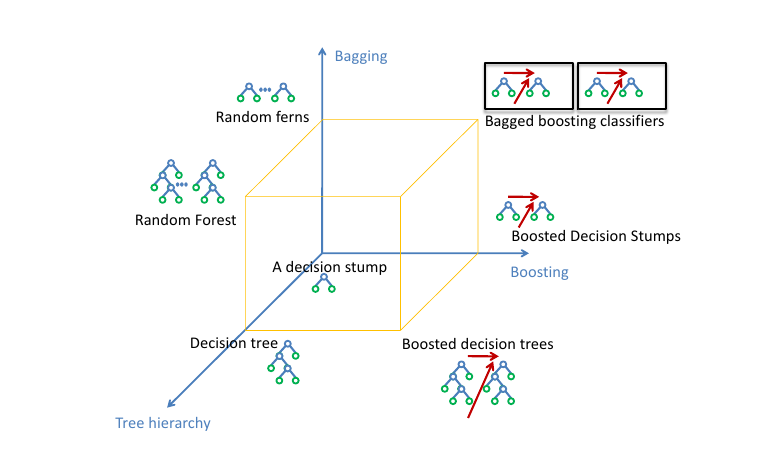
\includegraphics[width=\linewidth]{images/meta-algorithm-trees}
	\caption{Meta-Algoritmi applicati sui decision stump.}
\end{figure}


\section{Decision Trees}
Applichiamo la \textbf{tree hierarchy} sui nostri decision stump, ottenendo una gerarchia di decisioni. Tramite una serie di domande di tipo "yes/no", o varie sogliature, diventa possibile classificare categorie sempre più specifiche. Ogni coppia di risultati di un nodo di un decision tree, è detta \textit{split}. La profondità (direttamente proporzionale al numero di split), definisce la complessità del modello. Alberi decisionali troppo profondi rischiado di cadere in overfitting.

\section{Random Ferns}\label{sec:random_ferns}
Le \textbf{Random Ferns} sono una variante semplificata dei decision trees, progettata per essere particolarmente efficiente in termini di tempo di addestramento e predizione. Invece di costruire un albero completo con molteplici livelli di split, i random ferns consistono in un insieme di "ferns" (felce), ognuno dei quali è costituito da un numero fisso di stumps (domande binarie). Ogni fern è quindi una struttura piatta, senza gerarchia, che valuta un insieme di feature in parallelo.

Ogni fern produce una distribuzione di probabilità sulle classi target, basata sulle risposte alle domande binarie. La combinazione di più ferns permette di ottenere una stima complessiva della probabilità di appartenenza a ciascuna classe, rendendo questo approccio particolarmente adatto per compiti di classificazione rapida, come il riconoscimento di immagini.

\bigskip
\noindent
\textit{\textbf{Nota:} può essere trovato un approfondimento sulle Random Ferns nel capitolo \ref{chap:approfondimenti_teorici}, sezione \ref{sec:random_ferns_idea}.}

\section{Random Tree}
Un \textbf{Random Tree} è una variante del classico decision tree in cui la costruzione dell’albero non avviene in modo completamente deterministico, ma introduce una componente di casualità nella scelta degli split. 

Negli alberi decisionali standard, per ogni nodo si valutano sistematicamente tutte le possibili feature (e spesso tutte le possibili soglie) selezionando quella che massimizza la riduzione dell’impurità. In un random tree, invece, non si esplora l’intero spazio delle possibilità: si genera un insieme limitato di proposte casuali e si sceglie la migliore tra queste.

In particolare, ad ogni nodo:
\begin{itemize}
    \item si seleziona casualmente un sottoinsieme di feature candidate;
    \item per ciascuna feature si generano una o più soglie casuali;
    \item si valuta un criterio di qualità solo su queste proposte;
    \item si sceglie lo split che produce il miglior miglioramento secondo il criterio adottato.
\end{itemize}

La struttura dell’albero rimane quella di un decision tree classico, ma la procedura di costruzione è randomizzata. Questo rende il modello meno sensibile a piccole variazioni dei dati e particolarmente adatto a essere utilizzato all’interno di metodi ensemble come le Random Forest.

\subsection{Randomized Learning}

La costruzione del random tree avviene in modo ricorsivo. 

Dato un nodo associato a un insieme di indici $I_n$ (cioè i campioni che raggiungono quel nodo), si considera uno split basato su una funzione $f$ applicata ai vettori di feature $v_i$. Lo split è definito da una soglia $t$:

\[
I_l = \{ i \in I_n \mid f(v_i) < t \}
\qquad
I_r = I_n \setminus I_l
\]

dove:
\begin{itemize}
    \item $v_i$ è il vettore delle feature del campione $i$,
    \item $f$ è una feature candidata,
    \item $t$ è una soglia scelta casualmente nell’intervallo compreso tra il valore minimo e massimo assunto da $f(v_i)$ nel nodo corrente.
\end{itemize}

Lo scopo è suddividere i dati in due sottoinsiemi il più possibile omogenei rispetto alla variabile target.

\subsection{Guadagno di informazione}

Per valutare la qualità di uno split si utilizza una misura di impurità, indicata con $E(I)$ (come per esempio l'entropia). Il criterio di scelta si basa sulla riduzione di impurità, ossia sul \textbf{guadagno di informazione}:

\[
\Delta E
=
E(I_n)
-
\frac{|I_l|}{|I_n|} E(I_l)
-
\frac{|I_r|}{|I_n|} E(I_r)
\]

Questa quantità misura quanto l’incertezza nel nodo padre viene ridotta dallo split. Lo split selezionato è quello che massimizza $\Delta E$ tra le proposte generate casualmente.

Il processo viene poi applicato ricorsivamente ai nodi figli fino a quando si soddisfa un criterio di arresto (profondità massima, numero minimo di campioni, purezza del nodo, ecc.).

\subsection{Ruolo della casualità}
Un singolo decision tree è un modello ad alta varianza: piccole variazioni nei dati possono produrre alberi molto diversi. La randomizzazione:

\begin{itemize}
    \item riduce la correlazione tra alberi diversi;
    \item aumenta la diversità nei modelli;
    \item migliora la robustezza quando più alberi vengono combinati;
    \item riduce il rischio di overfitting.
\end{itemize}

Per questo motivo i random trees vengono spesso utilizzati come componenti di metodi ensemble, dove più alberi vengono addestrati su dati o feature diverse e le loro predizioni vengono aggregate (media o voto).

\subsection{Randomized Learning}

Il concetto di \textbf{randomized learning} consiste proprio nell’introdurre casualità controllata durante l’apprendimento per ottenere modelli meno correlati e più stabili quando combinati. Nel contesto del riconoscimento di immagini, la randomizzazione può riguardare:
\begin{itemize}
    \item la scelta delle feature;
    \item la scelta delle soglie;
    \item la struttura dell’albero;
    \item oppure la suddivisione dei dati (come nel bagging).
\end{itemize}

L’idea generale è che un singolo modello casuale possa essere debole o instabile, ma la combinazione di molti modelli randomizzati produce un sistema complessivamente più robusto ed efficace.

\section{Random forest}
Le random forest nascono dall'unione delle intuizioni relative al bagging e alla tree hierarchy. Si basano sulla combinazione di output di più decision trees (spesso random trees) per ottenere un unico risultato. La loro facilità d'uso e la  flessibilità ne hanno favorito l'adozione, e possono essere usate sia su task di classificazione che di regressione.  Offrono un ottimo grado di \textbf{precisione}, \textbf{cadono meno facilmente in overfitting} e sono assolutamente \textbf{multi-core friendly}.

\begin{figure}[tbph]
	\centering
	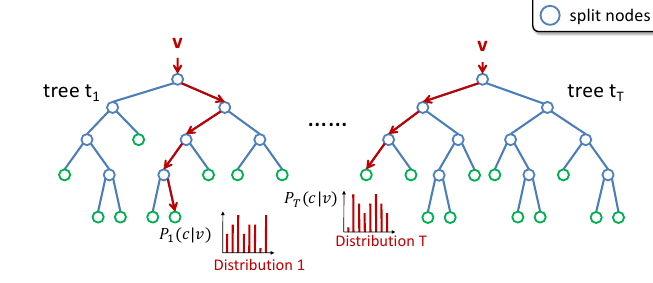
\includegraphics[width=1\linewidth]{images/random-forest}
\end{figure}

La classificazione è ottenuta considerando la distribuzione media computata dalle foglie.

$$
\frac{1}{T} \sum_{t=1}^{T}P_t(c|v)
$$

\section*{Riferimenti}
I riferimenti per questo capitolo includono:
\begin{itemize}
	\item Materiale visto a lezione.
	\item Random Ferns dal paper \citetitle{Ozuysal2008RandomFerns} \cite{Ozuysal2008RandomFerns}.
\end{itemize}